\documentclass[10pt,aspectratio=169]{beamer}
\usetheme[block=fill]{metropolis}

%\usepackage{graphicx}
\usepackage{verbatim}
\usepackage{animate}
\usepackage[english,ngerman]{babel}


\title{\centerline{\huge GPU Computing}}
%\subtitle{\centerline{\Large Arithmetics}}
\date{\centering 10. J\"anner 2020}
\author{\centerline{\large Christian M\"osl \\ Burhan Karababa}}
\institute{\centering \vspace*{0.5em} Department of Computer Sciences \\ University of Salzburg}

\setbeamersize{text margin left=2em}
\setbeamersize{text margin right=2em}

\begin{document}

\maketitle

\begin{frame}[standout]
    \alert{G}raphics \alert{P}rocessing \alert{U}nit - Computing
\end{frame}

\begin{frame}[fragile]{Aufgabe der Grafikkarte}
\begin{minipage}[t]{0.3\textwidth}
3 x 3 Pixel Bildschirm:
\begin{small}
    \begin{verbatim}
      framebuffer[3][3] = { 
        0x000102, 0x00000, 0xFFFFFF 
        0x0000FF, 0x00000, 0xAAAAAA
        0xBBBBBB, 0x00000, 0x000000 
      }
    \end{verbatim}
\end{small}
\end{minipage}
\begin{minipage}[t]{0.3\textwidth}
\vspace{1.5cm}
\begin{center}
\Huge $\qquad \Rightarrow$
\end{center}
\end{minipage}
\begin{minipage}[t]{0.3\textwidth}
\begin{figure}[ht]
    \begin{center}
        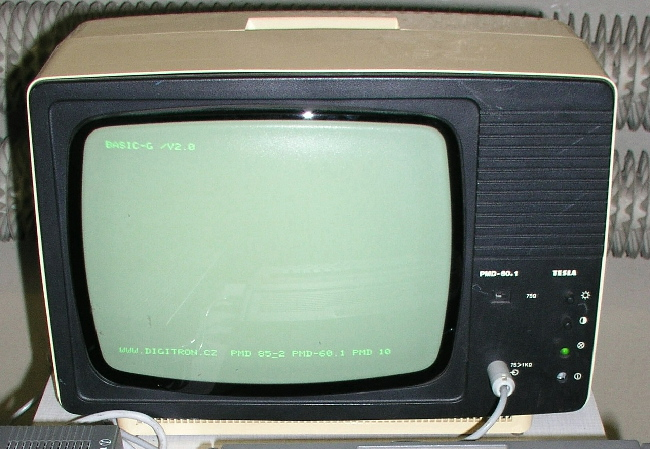
\includegraphics[width=0.9\textwidth]{crt.jpg}
    \end{center}
    \source{\footnotesize http://www.digitron.cz/galerie/original/ a\_PMD60-1b.jpg}
\end{figure}
\end{minipage}
\end{frame}

\begin{frame}{Grafikkarte aus 1985}
    \begin{figure}[ht]
        \begin{center}
            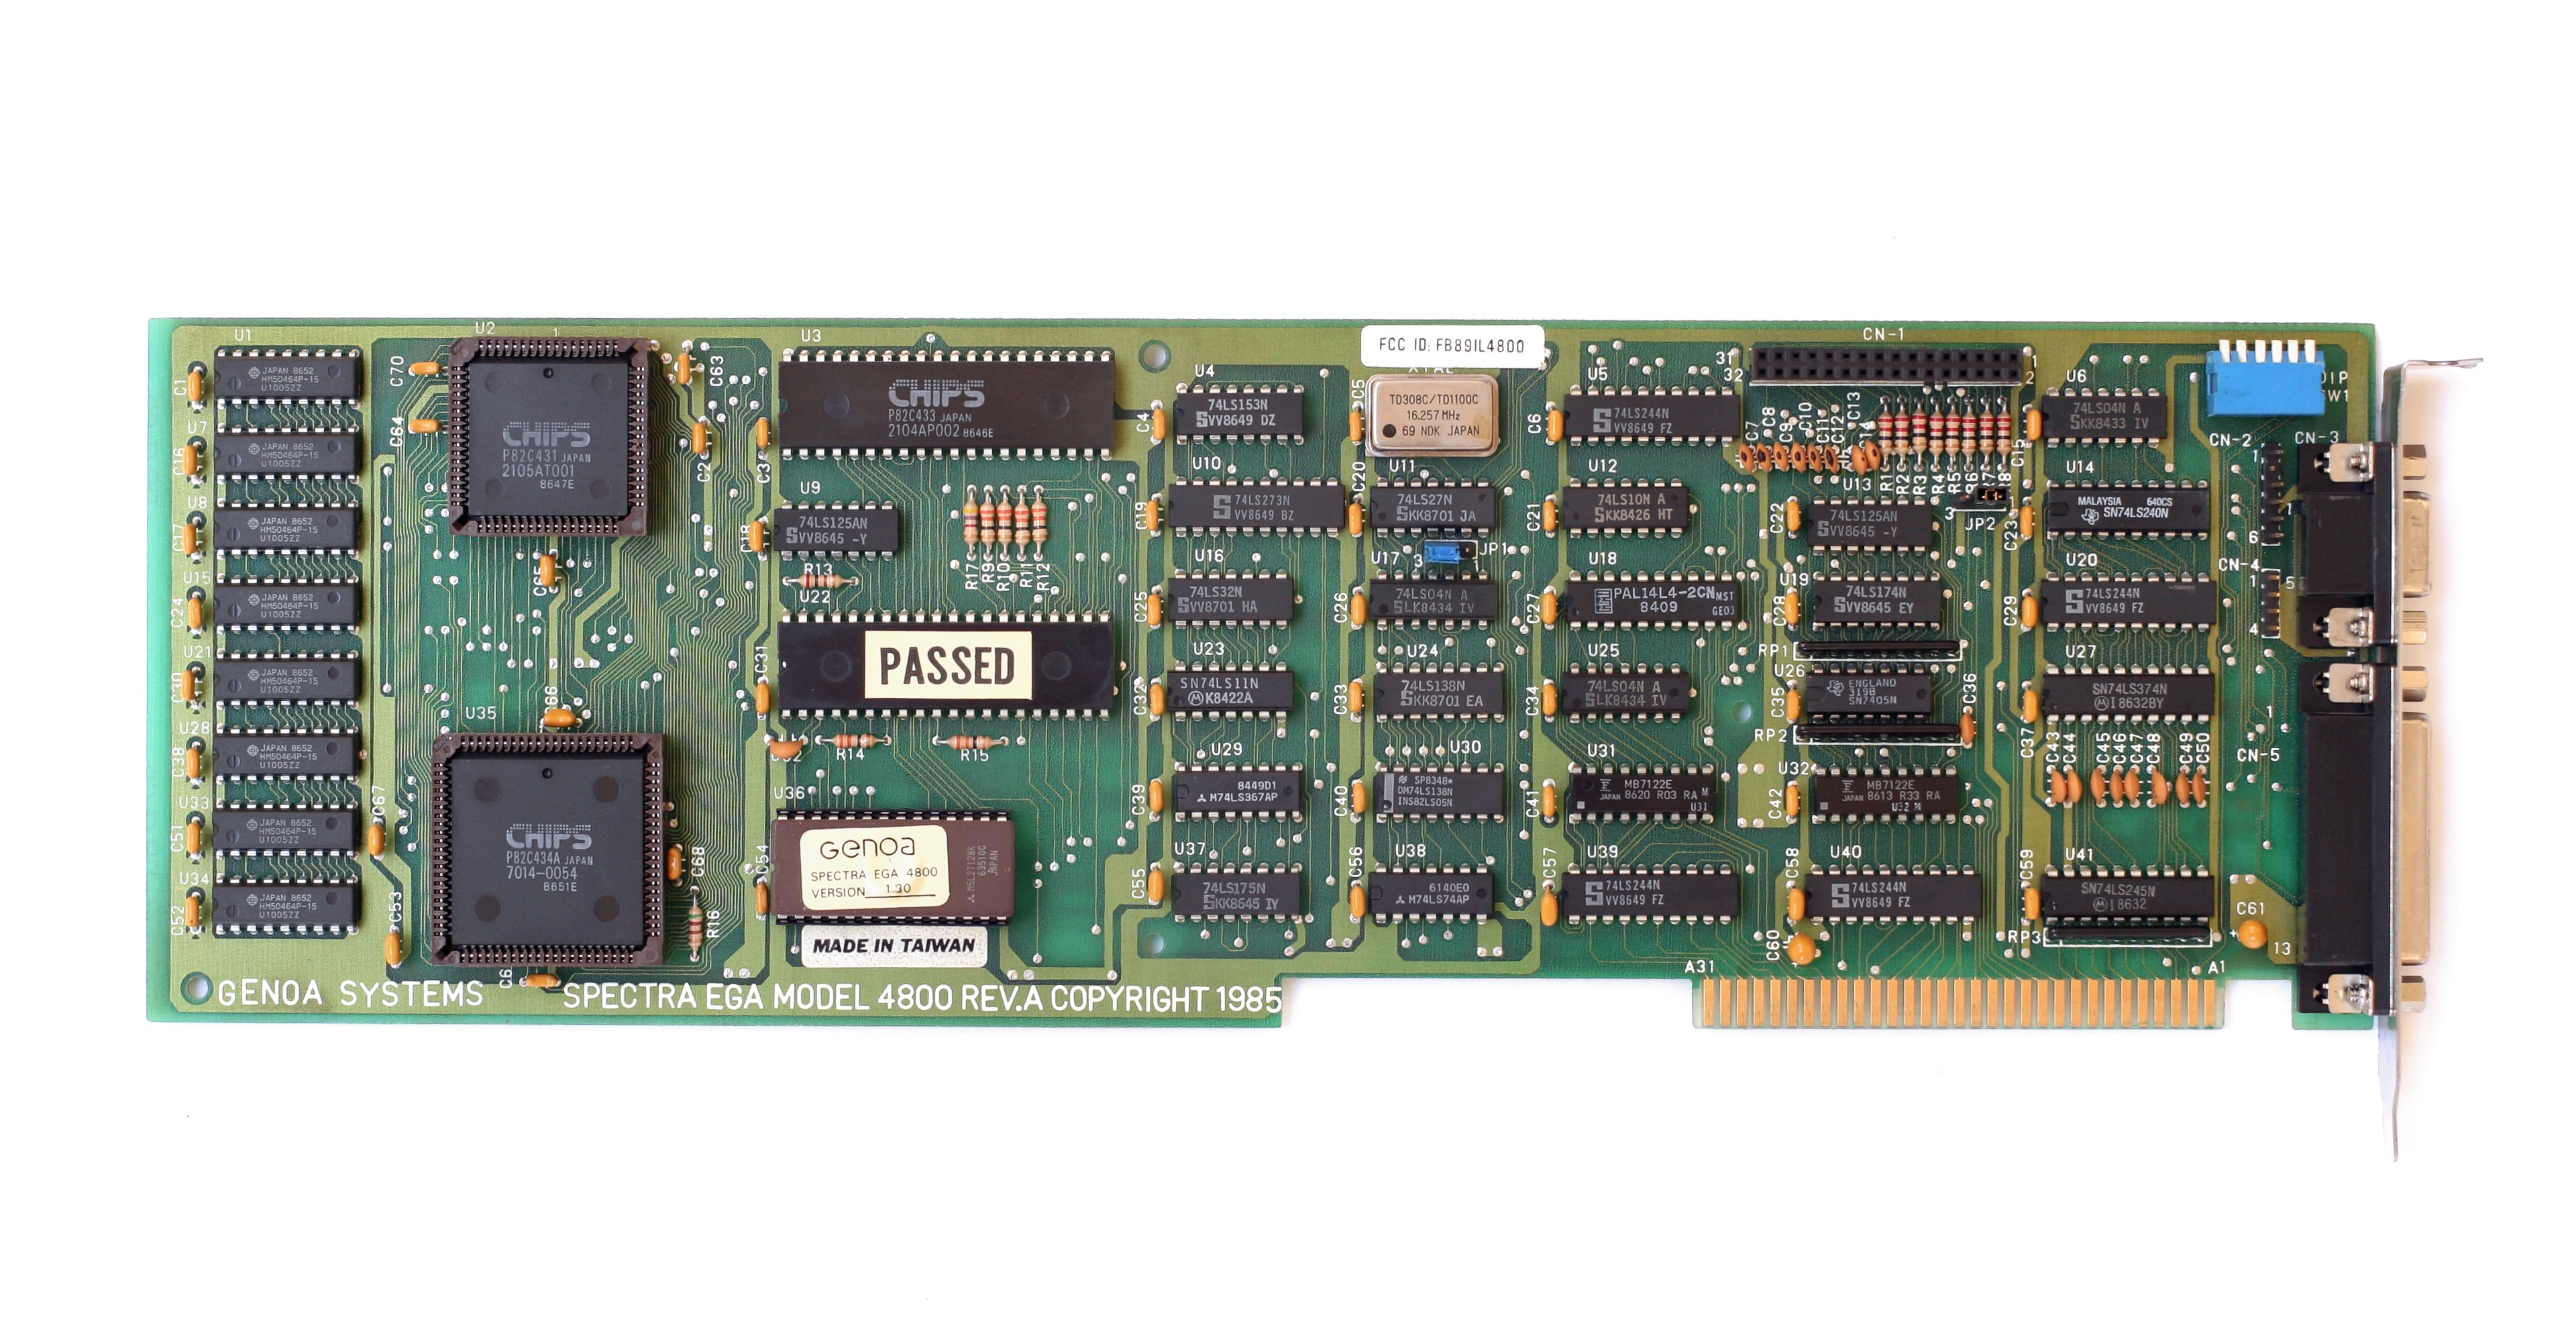
\includegraphics[width=0.9\linewidth]{KL_Genoa_EGA.jpg}
        \end{center}
        \source{\footnotesize https://de.wikipedia.org/wiki/Grafikkarte}
    \end{figure}
\end{frame}

\begin{frame}{2D Beschleuniger}
\begin{minipage}[t]{0.32\textwidth}

\includegraphics[width=0.9\textwidth]{cpu.png}
\end{minipage}
\begin{minipage}[t]{0.32\textwidth}
\vspace{-2cm}
$\quad \overset{drawLine(x, y, length, angle)}{\Rightarrow}$
\end{minipage}
\begin{minipage}[t]{0.32\textwidth}
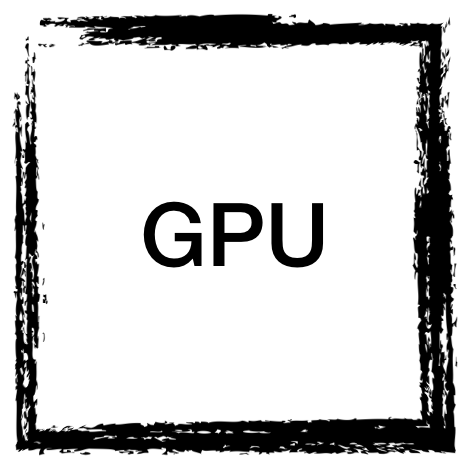
\includegraphics[width=0.9\textwidth]{gpu.png}
\end{minipage}
\end{frame}

\begin{frame}{3D Beschleuniger: Spiele}
  Rendering Problem: 

  \begin{itemize}
      \item Geometrie
      \item Texturen
      \item Licht
      \item Schattierung
      \item Perspektive
  \end{itemize}
\end{frame}

\begin{frame}{Parallelit\"at in Hardware}
    \begin{figure}[ht]
        \begin{center}
            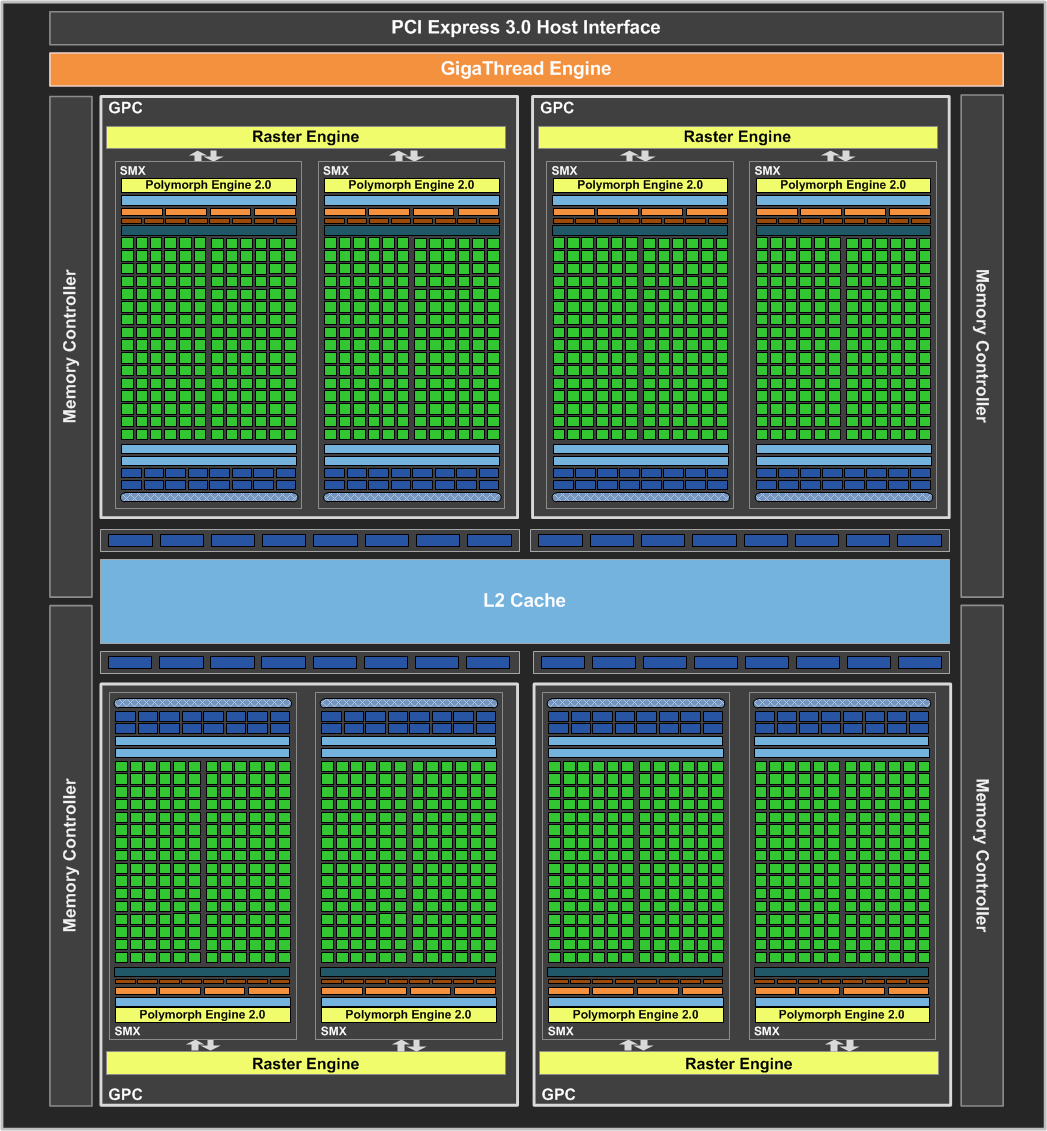
\includegraphics[height=0.8\textheight]{nvidia-pascal.png}
        \end{center}
        \source{\footnotesize https://images.anandtech.com/doci/5699/GeForce\_GTX\_680\_Block\_Diagram\_FINAL.png}
    \end{figure}
\end{frame}

\begin{frame}{FLOPS - eine Metrik}
    \begin{itemize}
        \item \textbf{Fl}oating Point \textbf{Op}eration \textbf{P}er \textbf{S}econd 
        \item arithmetische Operationen: +, -,...
        \item nicht überbewerten
    \end{itemize}
\end{frame}

\begin{frame}{CPU vs. GPU}
    \begin{figure}[ht]
        \begin{center}
            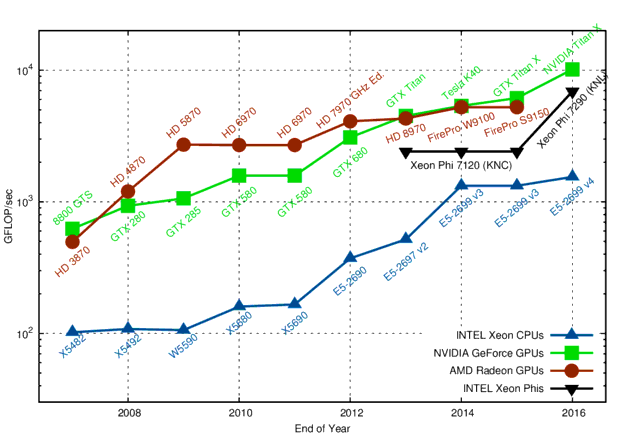
\includegraphics[height=0.8\textheight]{gflops.png}
        \end{center}
        \source{\footnotesize https://www.karlrupp.net/2013/06/cpu-gpu-and-mic-hardware-characteristics-over-time/}
    \end{figure}
\end{frame}

\begin{frame}{CPU vs. GPU}
    \begin{figure}[ht]
        \begin{center}
            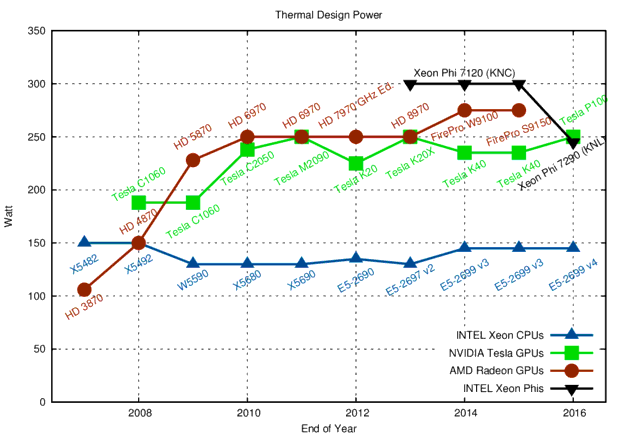
\includegraphics[height=0.8\textheight]{watt.png}
        \end{center}
        \source{\footnotesize https://www.karlrupp.net/2013/06/cpu-gpu-and-mic-hardware-characteristics-over-time/}
    \end{figure}
\end{frame}

\begin{frame}{Mythbusters Demo GPU versus CPU}
    \begin{figure}[ht]
       \href{https://www.youtube.com/watch?v=-P28LKWTzrI}{KLICK}
    \end{figure}
\end{frame}


\begin{frame}{GPU Computing: Mathematische Probleme}
    \begin{itemize}
        
        \item Lösung von Algorithmen/mathematischen Problemen
        \item Bewertung des Algorithmus aufgrund der Komplexität/Parallelisierungsgrad
        \item Arithmetische Berechnungen in der GPU/CPU?
        \item Embarrassingly-Parallel-problems und Inherently-serial-problems
    
        \end{itemize}
\end{frame}

\begin{frame}{Embarrassingly-parallel-problems}
    \begin{itemize}
 
        \item keine Abhängigkeiten zwischen einzelnen Schritten 
        \item Verarbeitungsschritte parallel durchführen
        \item Unterteilung in mehrerere kleinere Probleme
        \item kein Kommunikationsaufwand zwischen Prozessen notwendig
        \item benötigt mögichlicherweise Zusammenführung der Ergebnisse
        \item Beispiele: Matrizenrechnung, Password cracking
    
        
    \end{itemize}
\end{frame}

\begin{frame}{Inherently-serial-problems}
    \begin{itemize}

        \item keine Parallelisierbarkeit aufgrund von starken Abhängigkeiten
        \item benötigen Zwischenergebnisse um effizient weiterzuarbeiten
        \\ $ \rightarrow $ 
        z.B. Three-body-problem
      
    \end{itemize}
\end{frame}


\begin{frame}{GPGPU (General Purpose Computation on Graphics Processing Unit)}
    \begin{itemize}

\item Programmierschnittstelle: allgemeine Berechnungen von GPU auf Grafikkarte
\item Rechenleistung konsequent ausnutzen
\item Privatgebrauch: praktisch keine Anwendung für GPGPU (Ausnahme: Programme mit Videoverarbeitung)
\item Einsatzgebiet: Berechnung von wissenschaftlichen arithmetischen Problemen
\item 2007 Meilenstein: NVidia-Toolkit für die Programmierung von GPU's
  
\end{itemize}
\end{frame}


\begin{frame}{CUDA  - Toolkit}
    \begin{itemize}
       \item CUDA (Compute Unified Device Architecture): Wegbereiter GPU Computing
       \item von Nvidia entwickelte Programmier-Technik $ \rightarrow $ Bereitstellung Rechenkapazität
       \item entwickelt für wissenschaftliche Programmierungen
        \item nur für Einsatz auf NVidia-Karten $ \rightarrow $ herstellerabhängig
        \item Erweiterung der Sprache C/C++ $ \rightarrow $ geringe Einarbeitungszeit, keine Grafikkenntnisse notwendig
      


    \end{itemize}
\end{frame}

\begin{frame}{OpenCL - Toolkit}
    \begin{itemize}
\item OpenCL (Open Computing Language): offener Standard für Implementierung aller Typen von GPU's
\item 2008 zum ersten Mal als Standard eingereicht von AMD, IBM, Intel
\item Erweiterung der Sprache C/C++ (wie CUDA)
\item Installation von Treiber und Bibliotheken sehr komplex
\item Schwierigkeiten bei Installation Linux $ \rightarrow $ mangelnde Integration der Installer


    \end{itemize}
\end{frame}


\begin{frame}{Anwendung: Folding@Home}
    \begin{itemize}
        \item Erforschung von Krankheiten (Alzheimer, Krebs) - Universität Stanford
        \item besseres Verständnis für Faltung von Proteinen $ \rightarrow $  Mechanismen erkennen
        \item eines der ersten Projekte die auch GPU's miteinbeziehen
         \item erreichte am 20. Mai 2016 eine Rechenleistung von über 100 PetaFLOPS
         \item CUDA-Technik und OpenCL
        \item seit Projektbeginn insgesamt  205 Publikationen (Stand 31. Dezember 2018)

    \end{itemize}
\end{frame}

\begin{frame}{Anwendung: Deep Learning}
    \begin{figure}[ht]
        \begin{center}
            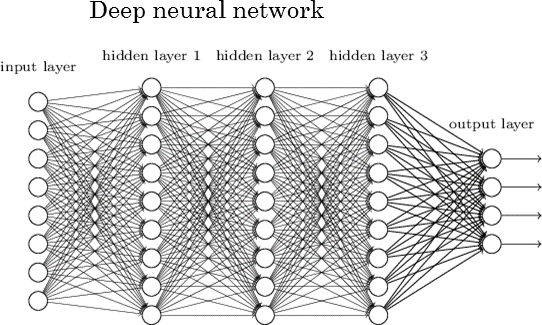
\includegraphics[height=0.8\textheight]{slide5.png}
        \end{center}
        \source{\footnotesize https://datawarrior.wordpress.com/2017/10/31/interpretability-of-neural-networks/}
    \end{figure}
\end{frame}


{
\usebackgroundtemplate{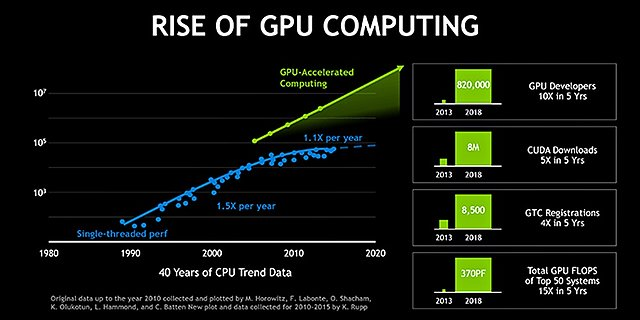
\includegraphics[width=\paperwidth]{nvidia-rise.jpg}}
\begin{frame}[plain]
\vspace{8cm}
\centering
\footnotesize{https://www.nvidia.com/de-de/about-nvidia/ai-computing/}
\end{frame}
}

\begin{frame}[standout]
   
Danke für eure Aufmerksamkeit!

\end{frame}

\end{document}